\subsection{Contextualização e tarefas do robô}
%TODO Elael: Caso JIRAU, contextualização (Ambiente), acessos à turbina
% (detalhar os acessor pela dimensão e etc) , tarefas do Robô e questoes
% relacionadas

A usina hidrelétrica de Jirau utiliza turbina do tipo bulbo, na qual um grande
bulbo com um gerador elétrico é submerso e acoplado a uma hélice horizontal do
tipo \textit{Kaplan}. Como a geração de energia depende da altura da queda
d'água e da vazão do rio, as turbinas do tipo bulbo utilizam uma grande vazão de
água para produzirem energia suficiente. A figura \ref{fig::bulb_turbine}
ilustra uma turbina do tipo bulbo e o grandes dutos necessários para comportar o
grande volume de água que passa através da turbina. 

\begin{figure}[h!]	
	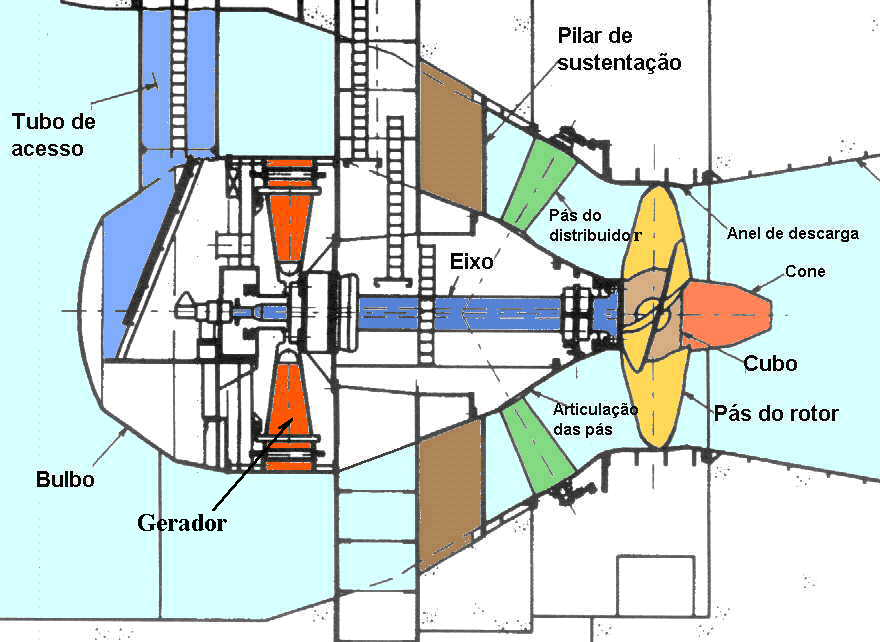
\includegraphics[width=\columnwidth]{figs/intro/bulb_turbine}
	\caption{Ilustração de uma turbina do tipo bulbo.}
	\label{fig::bulb_turbine}
\end{figure}

Utilizando-se os processos de metalização atuais, processando as pás da hélice
em um local exterior à turbina, é necessária a retirada de todo o aro câmara,
desmontagem completa do rotor e logística de transporte das pás até o local
desejado. Essa operação, caso necessite ser realizada, demandaria a mobilização
de diversas equipes de manutenção, operação de pórtico rolante e transporte,
além de impossibilitar a utilização da turbina durante várias semanas.

No contexto do projeto proposto, as partes de interesse da turbina são:

\begin{itemize}
  \item Hélice e pás;
  \item Aro Câmara e regiões adjacentes;
  \item Escotilhas de acesso;
  \item Duto de sáida;
\end{itemize} 

\subsubsection{Hélice e pás}
\begin{itemize}
  \item Provavelmente o perfil hidráulico da pá não será disponibilizado. Sensores são necessários para isso. Rijeza possui esses sensores. 
  É propriedade intelectual. Mas tem meios para conseguir.
  \item Parte superior só pela escotilha. Mas, primeiramente, ela não será
  recuperada/revestida. 
  \item Não há sobreposição das pás.
  \item Varia 29 total (14.5 para cada lado). Melhor estar totalmente aberta, por ser, possivelmente, a posição 
de melhor acesso.
  \item  Pode ser girada, porém não é tão simples. Melhor realizar procedimento frente e verso para depois girar a 
turbina. Minimizar o número de rotações.
   \item Existe erosão e cavitação e esses fenômenos são influenciados pela
variação de queda d'água. Estudos mostraram que com diferenças maiores de 12 metros, os problemas de cavitação são 
minimizados.  Há cavitação em ambos os lados da pá devido a presença de fenômenos de alta e baixa pressão.
\end{itemize}

\subsubsection{Aro Câmara e regiões adjacentes}
\begin{itemize}
  \item superfícies metalicas
  \item Aro câmara é plano porém estreito
  \item Altura até o miolo do rotor de aprox 2,5m
  \item Região a montante do aro camara deve ser acessada passando-se pelo aro
  camara e helice
  \item Região a montante do aro camara inclinada, presença do distribuidor
  \item Regiao a jusante do aro camara também inclinada
\end{itemize}

\subsubsection{Escotilhas de acesso}
\begin{itemize}
  \item Inferior - acesso humano e equipamentos
    \item Menor escotilha de acesso da usina tem 80 cm
  	\item Escotilhas de acesso em posições diferentes dependendo da margem
  \item Superior - visualização do Lip da pá.
  \item Superior localiza-se no aro camara. 
\end{itemize}





